\documentclass[10pt,twocolumn,letterpaper]{article}

\usepackage{iccv}
\usepackage{times}
\usepackage{epsfig}
\usepackage{graphicx}
\usepackage{amsmath}
\usepackage{amssymb}

% Include other packages here, before hyperref.

% If you comment hyperref and then uncomment it, you should delete
% egpaper.aux before re-running latex.  (Or just hit 'q' on the first latex
% run, let it finish, and you should be clear).
\usepackage[pagebackref=true,breaklinks=true,letterpaper=true,colorlinks,bookmarks=false]{hyperref}

% \iccvfinalcopy % *** Uncomment this line for the final submission

\def\iccvPaperID{****} % *** Enter the ICCV Paper ID here
\def\httilde{\mbox{\tt\raisebox{-.5ex}{\symbol{126}}}}

% Pages are numbered in submission mode, and unnumbered in camera-ready
\ificcvfinal\pagestyle{empty}\fi
\begin{document}

%%%%%%%%% TITLE
\title{SCNN: Shape Constrained Neural Network for Membrane Structure Segmentation via Joint Pooling Operation}

\author{First Author\\
Institution1\\
Institution1 address\\
{\tt\small firstauthor@i1.org}
% For a paper whose authors are all at the same institution,
% omit the following lines up until the closing ``}''.
% Additional authors and addresses can be added with ``\and'',
% just like the second author.
% To save space, use either the email address or home page, not both
\and
Second Author\\
Institution2\\d
First line of institution2 address\\
{\tt\small secondauthor@i2.org}
}

\maketitle
%\thispagestyle{empty}


%%%%%%%%% ABSTRACT
\begin{abstract}
   Accurate segmentation of biomembrane structure is a crucial step to obtain morphological statistics in biomedical analysis.
   However in many scenarios, prior shape knowledge about biomedical objects is available, which is especially useful for segmenting dense and regular objects.
   In this paper, we introduce a new approach, named shape constrained neural network(SCNN), by incorporating prior shape knowledge about plausible components into neural network.
   Our SCNN is a multi-task learning framework that simultaneously predicts coarse segmentation map and parameterized contour expressions map as auxiliary.
   The auxiliary information are utilized to optimize the contour shape of each object, especially for regular objects.
   %As prior shape knowledge is represented by different contour expression form, segmentation map can be further improved.
   Moreover, a novel joint pooling operation is developed as a trainable layer to selectively express some predictions, which is both beneficial to multi-outputs.
   The whole process is efficient and optimized end-to-end.
   Experiments on synaptic vesicle segmentation and scene glands segmentation demonstrate the effectiveness of our approach.
   And we expect our method to empower more works to incorporate various shape constraints into segmentation tasks through deep convolutional neural networks.
   Code is made publicly available at \url{https://github.com/mboboUSTC/SCNN.git}.

\end{abstract}

%%%%%%%%% BODY TEXT
\section{Introduction}
Recent advances in biomedical image analysis have assisted many pathologists and biologists to facilitate their researches \cite{Xu2016}, \cite{Ronneberger2015}, \cite{Chen2016c}, \cite{Lieman-Sifry2017}, \cite{Paszke2016}.
Among these researches, a significant application is to obtain the accurate segmentation of specific membrane structure in a biomedical image, such as lumenal glands, synaptic vesicles and cells.
Especially, the morphological shape and spatial distribution of synaptic vesicles is helpful to study the neural activity in different brain regions, while [copy] morphological statistics of lumenal glands has been routinely used to assess the malignancy degree of adenocarcinomas.[copy]
Conventionally, these crucial steps are performed by human expert, which are time-consuming and suffer from subjective factors.
[copy]Therefore automatic segmentation methods are highly demanded to improve the efficiency as well as reliability and reduce the workload on experts[copy].

\begin{figure}\label{FigImgs}
\begin{center}
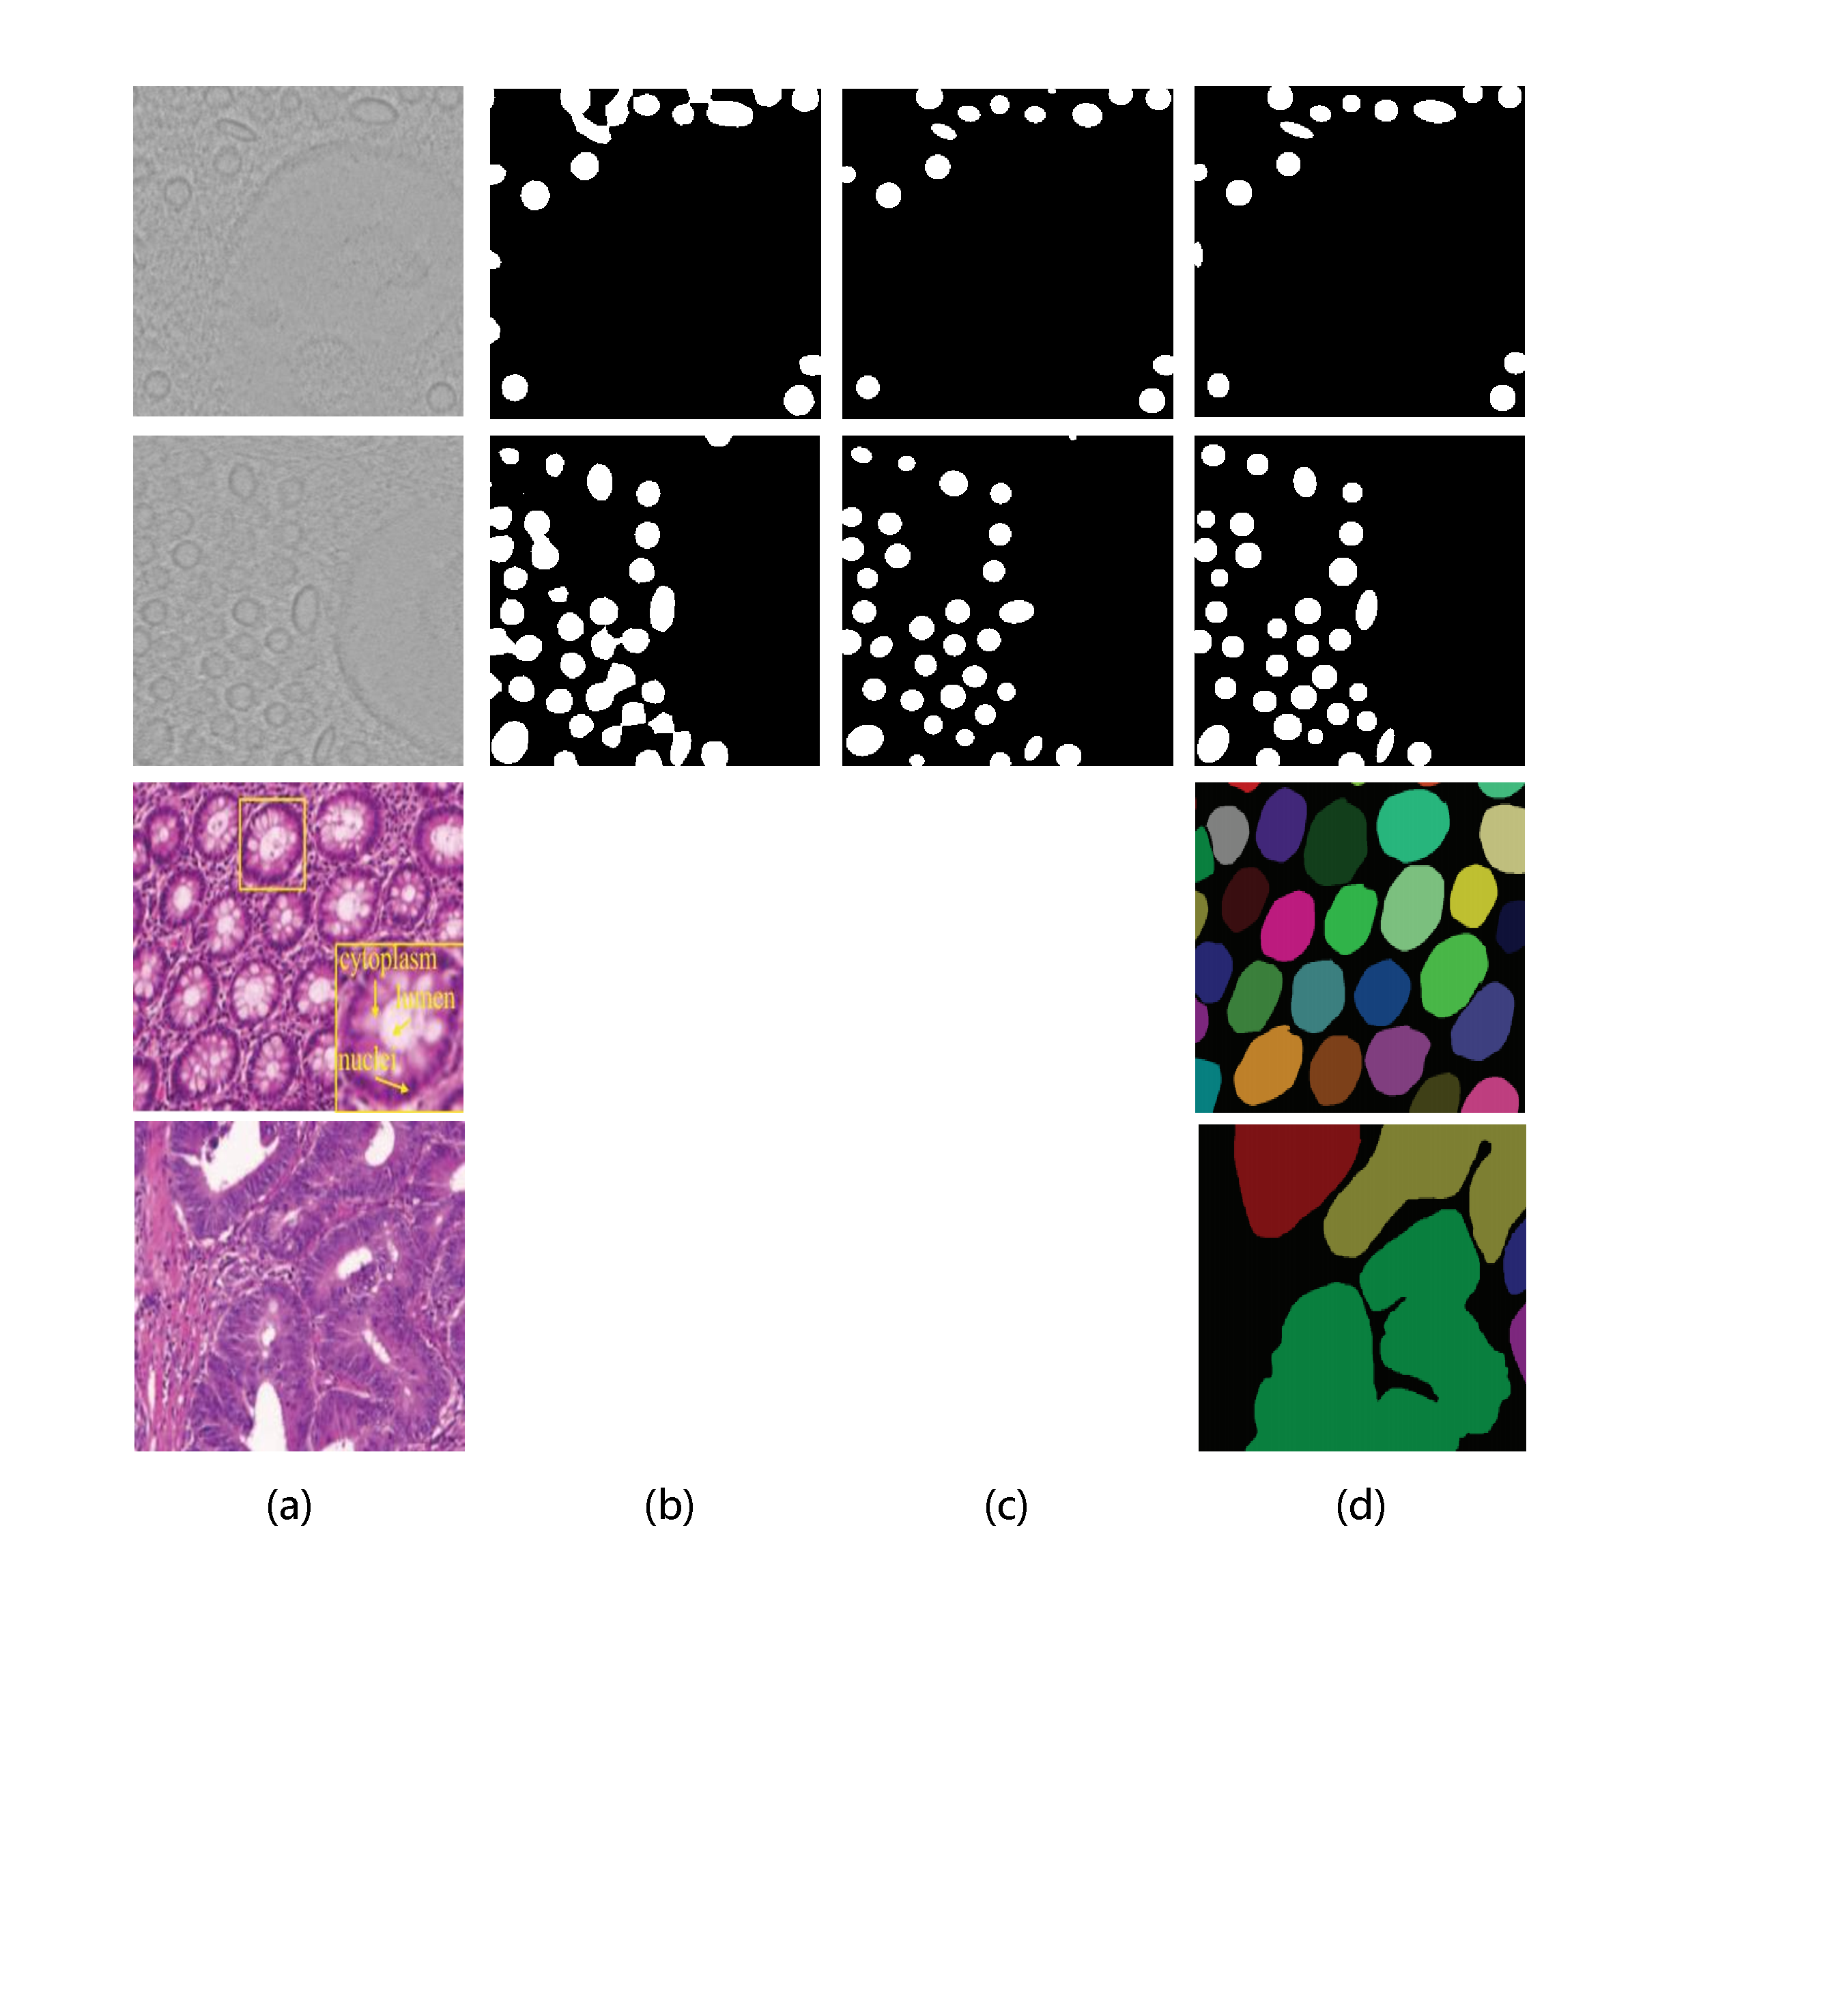
\includegraphics[width=3.3in]{Fig1.pdf}
\end{center}
   \caption{Examples illustrating deficiency of existing methods for biomedical segmentation. First two rows are dense synaptic vesicle with regular shape, and bottom two rows are benign and malignant gland. (a) biomedical image; (b) results from DCAN; (c) results from SCNN by incorporating prior shape constraint; (d) annotations by experts.}
\end{figure}

[copy]However, there exists several challenges in these tasks.[copy]
First, biomedical images are usually noisy and low contrast, because of deficient imaging technique as shown in Figure \ref{FigImgs} (left column).
Second, due to compact and dense arrangement of majority membrane structures, it is hard to separate objects individually, which is known as touching problem.
Third, as most deep neural architecture of biomedical images are based on fully convolutional networks \cite{Long2015}, they inevitably suffer from poor localized object boundaries caused by large receptive fields and many pooling layers.

Recently, deep neural networks have demonstrated excellent performance in biomedical image segmentation with the use of fully convolutional networks \cite{Long2015}, \cite{Dhungel2015}, \cite{Ronneberger2015}, \cite{Roth2015}, \cite{Chen2015}, \cite{Lieman-Sifry2017}, \cite{Xu2016}.
However, [copy]due to the employment of max-pooling and downsampling, the output of these networks tend to have poorly localized object boundaries[copy].
For this reason, [copy]\cite{Ronneberger2015} proposed the U-net that designed a U-shaped deep convolutional network for biomedical image segmentation.[copy]
[copy]It uses skip connections between the contracting and expanding paths to directly propagate context information to higher resolution layers to preserve details.[copy]
Later, a UNet variant, DeepVentricle \cite{Lieman-Sifry2017}, has been used for cardiac segmentation, which used same padding instead of valid padding.
Further improvements have been shown in DCAN \cite{Chen2016a}, which [copy]investigates the complementary information of objects and contours under a multi-task learning framework.[copy]
Specially, [weak copy]DCAN simultaneously segment the object and separate the clustered objects into individual ones with the help of their contours[weak copy].
Although these methods achieved promising results in their segmentation task, they may fail to achieving satisfying performance in denser, smaller objects with regular shape as shown in Figure 1.
Exactly, segmenting synaptic vesicles in our task raises higher demand on localizing contour for each vesicles.
\begin{figure}\label{FigMTN}
\begin{center}
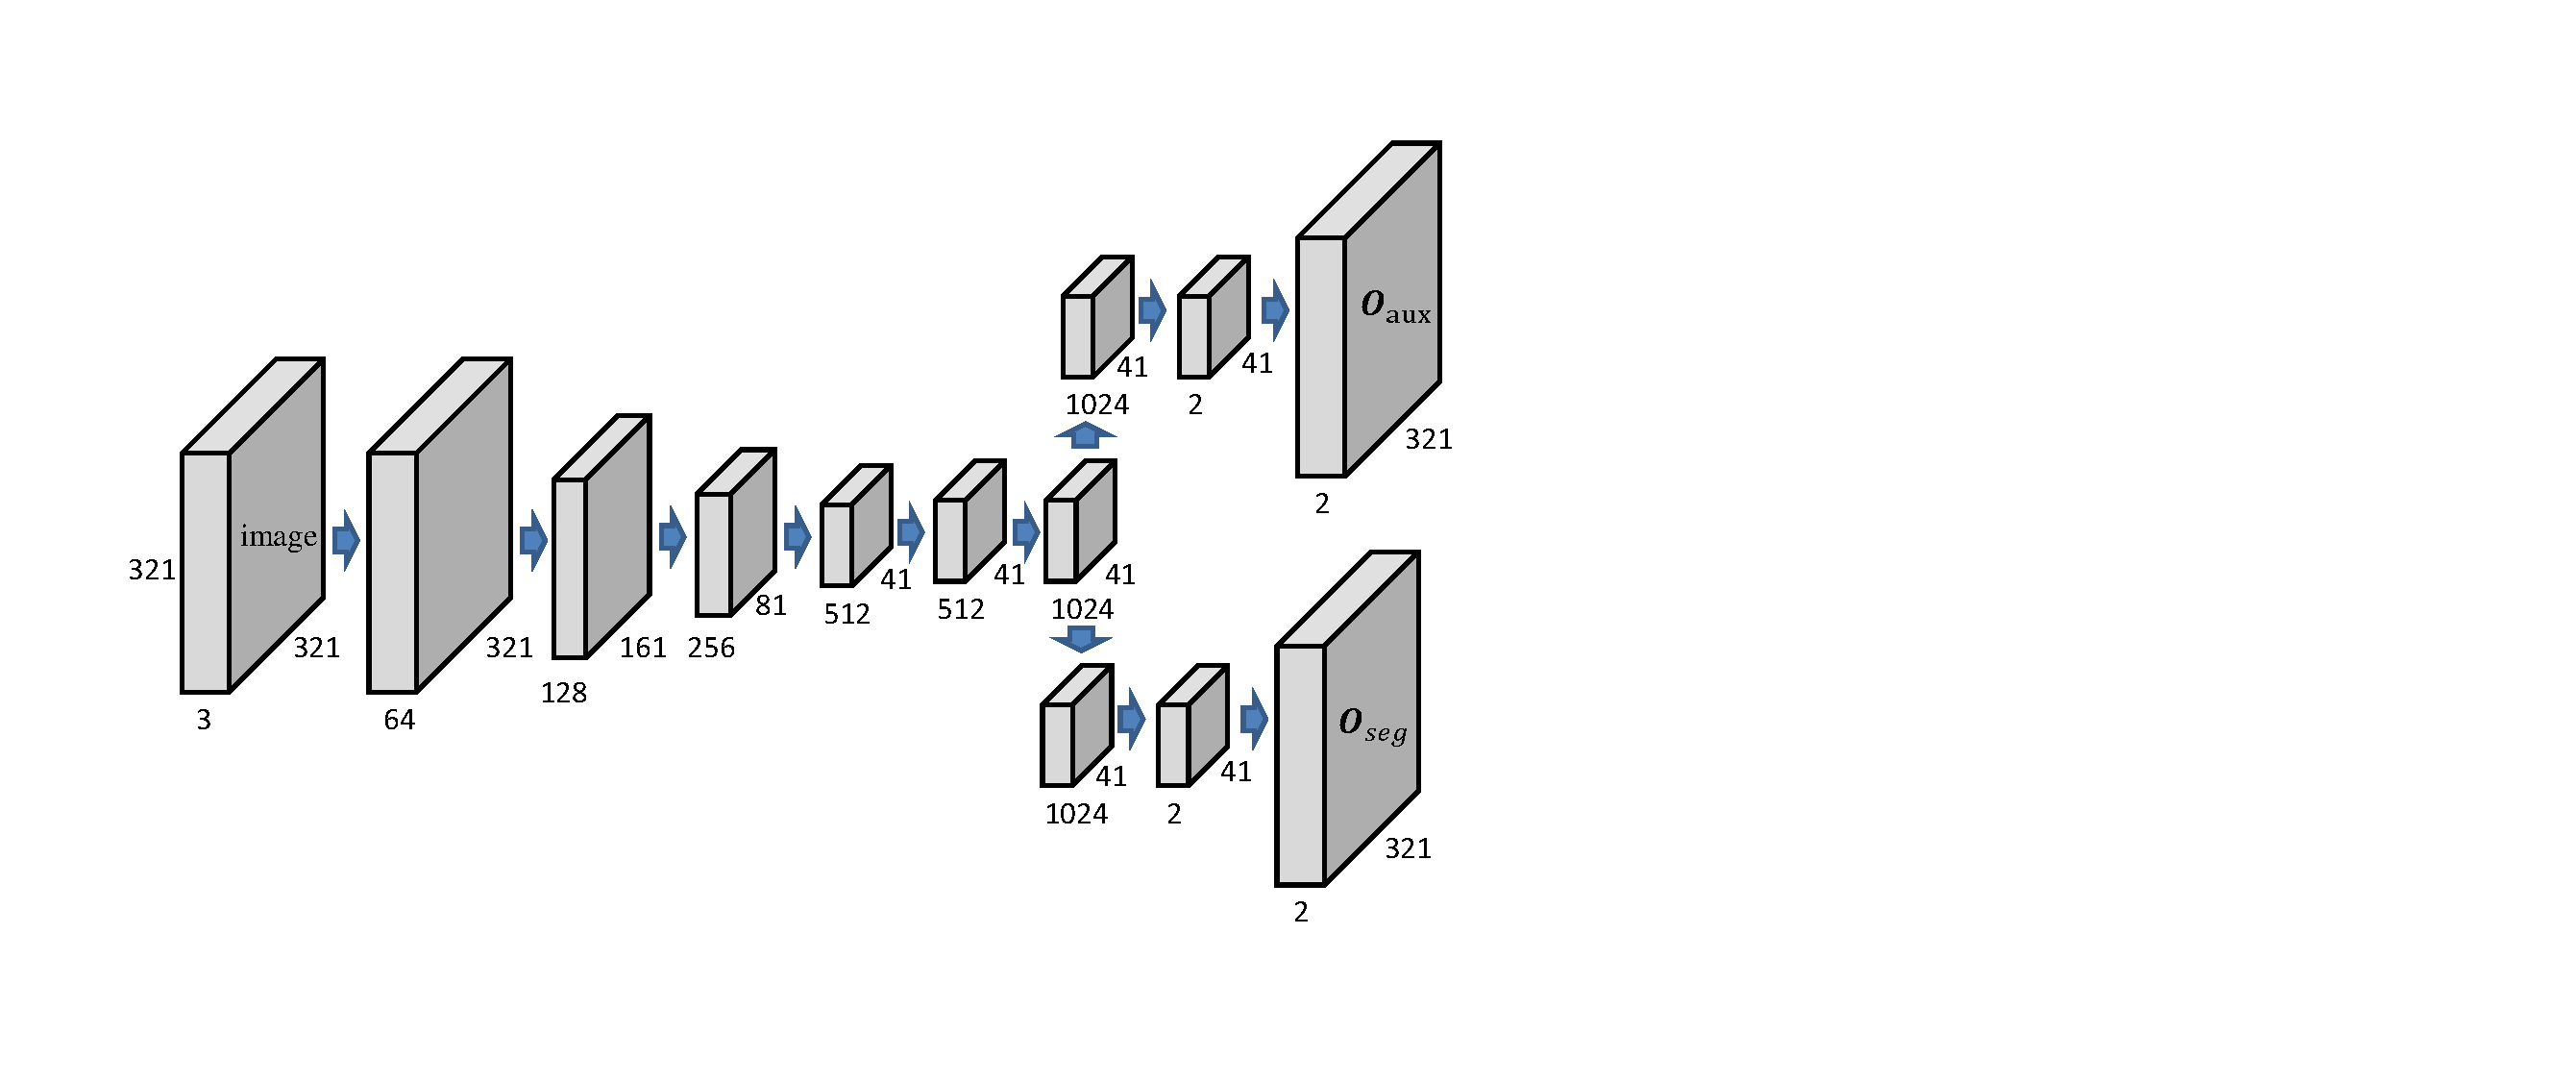
\includegraphics[width=3.3in]{FigMTN.pdf}
\end{center}
   \caption{The illustration of our multi-task network architecture.}
\end{figure}

\begin{figure*}\label{FigSCNN}
\begin{center}
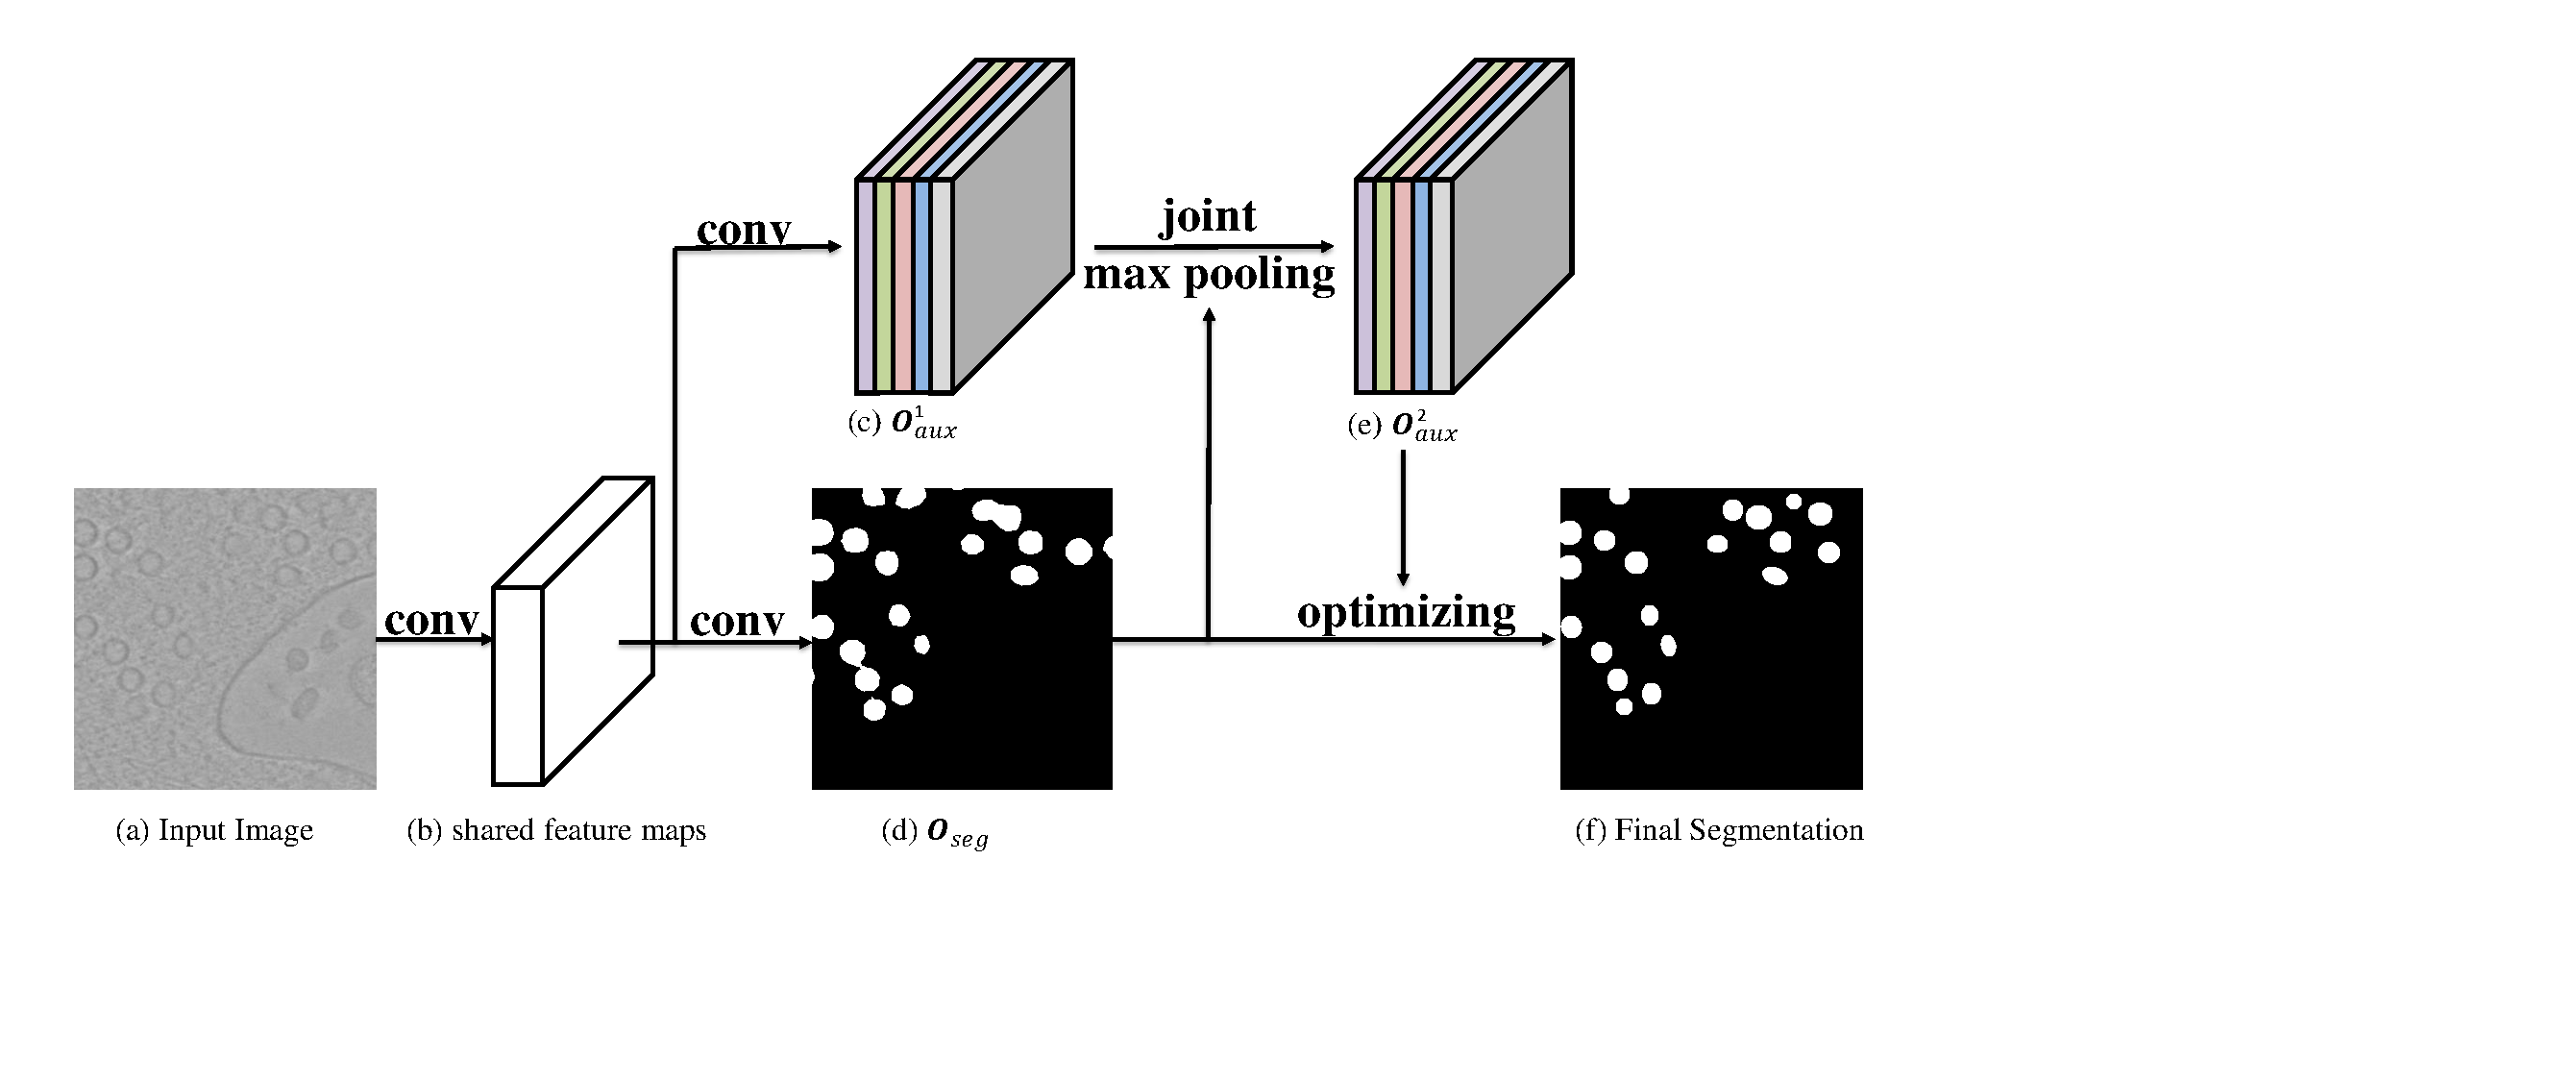
\includegraphics[width=6.8in]{Fig2.pdf}
\end{center}
   \caption{Overview of our proposed scnet. Given an image (a), multi-task neural network simultaneously predict a coarse segmentation (d) and parameterized contour description (d) using shared feature maps (b).
   Then a joint max pooling is applied to pool (c) with (d) and output new parameterized contour description (e).
   Finally, segmentation (f) is obtained by optimizing coarse segmentation (d) with the parameterized contour description (e).}
\end{figure*}

In this paper, we propose the first shape constraint neural network (SCNN) to segment dense objects by inherently incorporating prior shape knowledge into the network.
%while still accommodate serious shape deformation.
Similar to \cite{Chen2016a}, we formulate the network as a multi-task learning framework by simultaneously predicting a segmentation map and an auxiliary map.
%The auxiliary map, usually being contours map \cite{Chen2016a}, \cite{Chen2016}, \cite{Bertasius2016} ,is used to supplement complementary information for segmentation map.
Instead of predicting contour probability map, as used in \cite{Chen2016a}, \cite{Chen2016}, \cite{Bertasius2016}, our SCNN learn a parameterized description of contour shape as auxiliary map, which emphasizes more on overall shape of object.
%^In our framework, instead of directly predicting object contours, our SCNN learn the parameterized expression of contours, which emphasizes more on the overall shape of object.
%Especially, our parameterized contour expression can not only separate objects into individual ones, but also be embed in different shape constraint by defining different parameter composition.
The complementary information in parameterized contour description can not only separate objects into individual ones, but also optimize the contours shape..
However since there existing some seriously deformable objects, contours shape can't be parameterized uniformly and accurately.
To this end, we select a best representative shape as constrain and only modify segmentation predictions in ambiguous region, where usually contains contours, using the predicted parameterized contour description.
%In this way, most biomedical objects with regular shape, such as ellipse, are beneficial, while the segmentation of fractional deformable object are not obviously affected.

However, predicting parameterized contours description over the whole map is a much tougher task than contour probability map.
%Eespecially predictions within one object region it is hard to guarantee the predictions belonging to one object corresponding to an identical shape, and performance will drop obviously in contours area, which is the exact the area where we desire to modify the segmentation result.
Therefore, we proposed a novel joint max pooling (JMP) to only predict the contour description in center region of objects and fill the rest region with them.
Furthermore, JMP is designed as a trainable layer, of which the back propagation is benefit to both segmentation and parameterized contours description.
%Furthermore, it is designed as a trainable layer, which can be extended to any networks.
%Explicitly, the objectness map can be used to substitute the contours expressions belonging to one object region with the expression of the highest objectness score, which reduces the learning difficulties and improve the inference accuracy.
%And contours expression map will increase the penalties on objectness loss of the regions, where there exist disagreements between objectness prediction and parameterized countour prediction in trun.
%Our JMP can be implemented as a layer, which can be trained end-to-end and adopted to other multi-task networkds.

The contribution of this paper are:
1) effectively incorporating shape constraint into deep neural networks for biomedical image segmentation,
2) joint max pooling for benefiting both multi-task outputs,
3) achieving better performance on diverse biomedical segmentation tasks,
4) in experiments, we show that our method can be extended to scent detection task, which obtains the state of art performance
\section{Proposed Method}
A complete pipeline of Shape Constrained Neural Network (SCNN) is illustrated in Figure \ref{FigSCNN}.
The framework is trained end-to-end and consists of three key components:
1) a multi-task neural network based on FCN,
2) proposed joint max pooling and
3) optimizing segmentation result with parameterized contour description.
%First, we start by introducing our multi-task neural network in Sec. \ref{Sec21}.
%And then, joint max pooling is described in detail as a tainable layer in Sec. \ref{Sec22}.
%Finally, we show how to utilize the complementary information of parameterized contour expressions to improve segmentation performance in Sec. \ref{Sec23}.
\subsection{Multi-task FCN}
Due to essential ambiguity in touching regions caused by segmentation map, complementary information is needed to separate clustered objects into individuals ones.
In this section, we proposed a multi-task learning framework that simultaneously explore segmentation map $\mathbf{O}_{seg}$ and auxiliary map $\mathbf{O}_{aux}$ to provide complementary information.
A detailed description of network architecture is shown in Figure \ref{FigMTN}.

In this network, the feature learning part is shared and based on the publicly available DeepLab model \cite{Chen2014a}, which introduces zeros into the filters to enlarge its Field-Of-View.
It is initialized from VGG-16 ImageNet pretrained model.
Subsequently, feature maps output by last shared conv layer are fed into two individual branches.
In each branch, successive two conv layers, respectively with kernel size of $3\times3$ and $1\times1$, are applied to input map, and then an upsampling layer restore their resolution to the input image's.
%Especially, one branch predicts $\mathbf{O}^1_{seg}$ as a dense classification task, and the other branch predicts $\mathbf{O}^1_{aux}$ as a regression task.
During training, the parameters of shared network are jointly optimized, [copy] while the parameters of two individual branches are updated independently.

Instead of directly predicting contour probabilities \cite{Chen2016a}, \cite{Xu2016}, we choose parameterized contour description as our complementary information, which emphasizes more on the overall shape.
Especially, we use five parameters: $\theta^*$, $x_c^*$, $y_c^*$, $a^*$, $b^*$ to depict an ellipse shape.
$\theta^*$ is the rotated angle of major axis.
$x_c^*$, $y_c^*$ are the ellipse center coordinates.
And $a^*$, $b^*$ are respectively major and minor axis.
Different definitions of parameters means different shape prior knowledge of object contour.
Similar to \cite{Redmon2016}, the predicted contour description on $(x,y)$ is expressed by $\mathbf{O}_{aux}(x,y) = [\theta, dx_c, dy_c, a, b]$, where
\begin{eqnarray}\label{EqMax}
\begin{aligned}
\theta &= \theta^*\\
dx_c &= (x-x_c^*)/width\\
dy_c &= (y-y_c^*)/height\\
a &= a^*/width\\
b &= b^*/height\\
\end{aligned}
\end{eqnarray}
[$\theta^*$, $x_c^*$, $y_c^*$, $a^*$, $b^*$] are parameters depicting the true ellipse shape of the object to be segmented.
$width$ and $height$ are image size.

The objective function follows the multi-task loss in Faster R-CNN \cite{Ren2015}.
Our loss function for an image is defined as:
\begin{eqnarray}\label{EqLoss}
\begin{aligned}
L(\mathbf{O}_{seg},\mathbf{O}_{aux}) &= L_{seg}(\mathbf{O}_{seg},\mathbf{O}_{seg}^*)+\\
&\lambda L_{aux}(\mathbf{O}_{aux},\mathbf{O}_{aux}^*��\mathbf{O}_{seg})
\end{aligned}
\end{eqnarray}
where $L_{aux}(\mathbf{O}_{aux},\mathbf{O}_{aux}^*��\mathbf{O}_{seg}^*)$ only compute loss on regions with positive $\mathbf{O}_{seg}^*$ and $\lambda$ is a balancing weight.
\subsection{Joint Max Pooling}
In this section, we proposed a novel joint max pooling (JMP) to further improve both the accuracy of segmentation and parameterized contour predictions.
Different from conventional max pooling, our JMP takes two inputs and pooling one with the other one.
%JMP takes in the two outputs from previous multi-task neural networks and outputs two new predictions, as shown in Figure \ref{Fig_scnet}.

In a conventional pooling operation, the pooling operation can expressed by:
\begin{eqnarray}\label{pooling}
\begin{aligned}
y_{\mu,\nu} = \sum_{i,j}x_{i,j}s_{i,j}~~~~~~~x_{i,j}\in \mathbf{\overline{X}},s_{i,j}\in \mathbf{S}
\end{aligned}
\end{eqnarray}
where $\mathbf{\overline{X}}$ is the pooling window sliding on input map, and $\mathbf{S}$ is a weight matrix with the same size of $\mathbf{\overline{X}}$ .
Specifically for max pooling, $\mathbf{S}$ in Eq. \ref{pooling} is a binary matrix, whose elements are all zero except for the position which has a maximum $x$ in $\mathbf{\overline{X}}$.
When Eq. \ref{pooling} is an average pooling, all elements in $\mathbf{S}$ are identical averaging coefficient.
Intuitively, $\mathbf{S}$ acts like an "indictor" determining which information in $\mathbf{\overline{X}}$ should be propagated to next layer.
Based on this observation, we proposed a split version of pooling by obtaining $\mathbf{S}$ from an independent input, instead of $\mathbf{\overline{X}}$.
%This novel split.
\begin{figure}\label{FigJMP}
\begin{center}
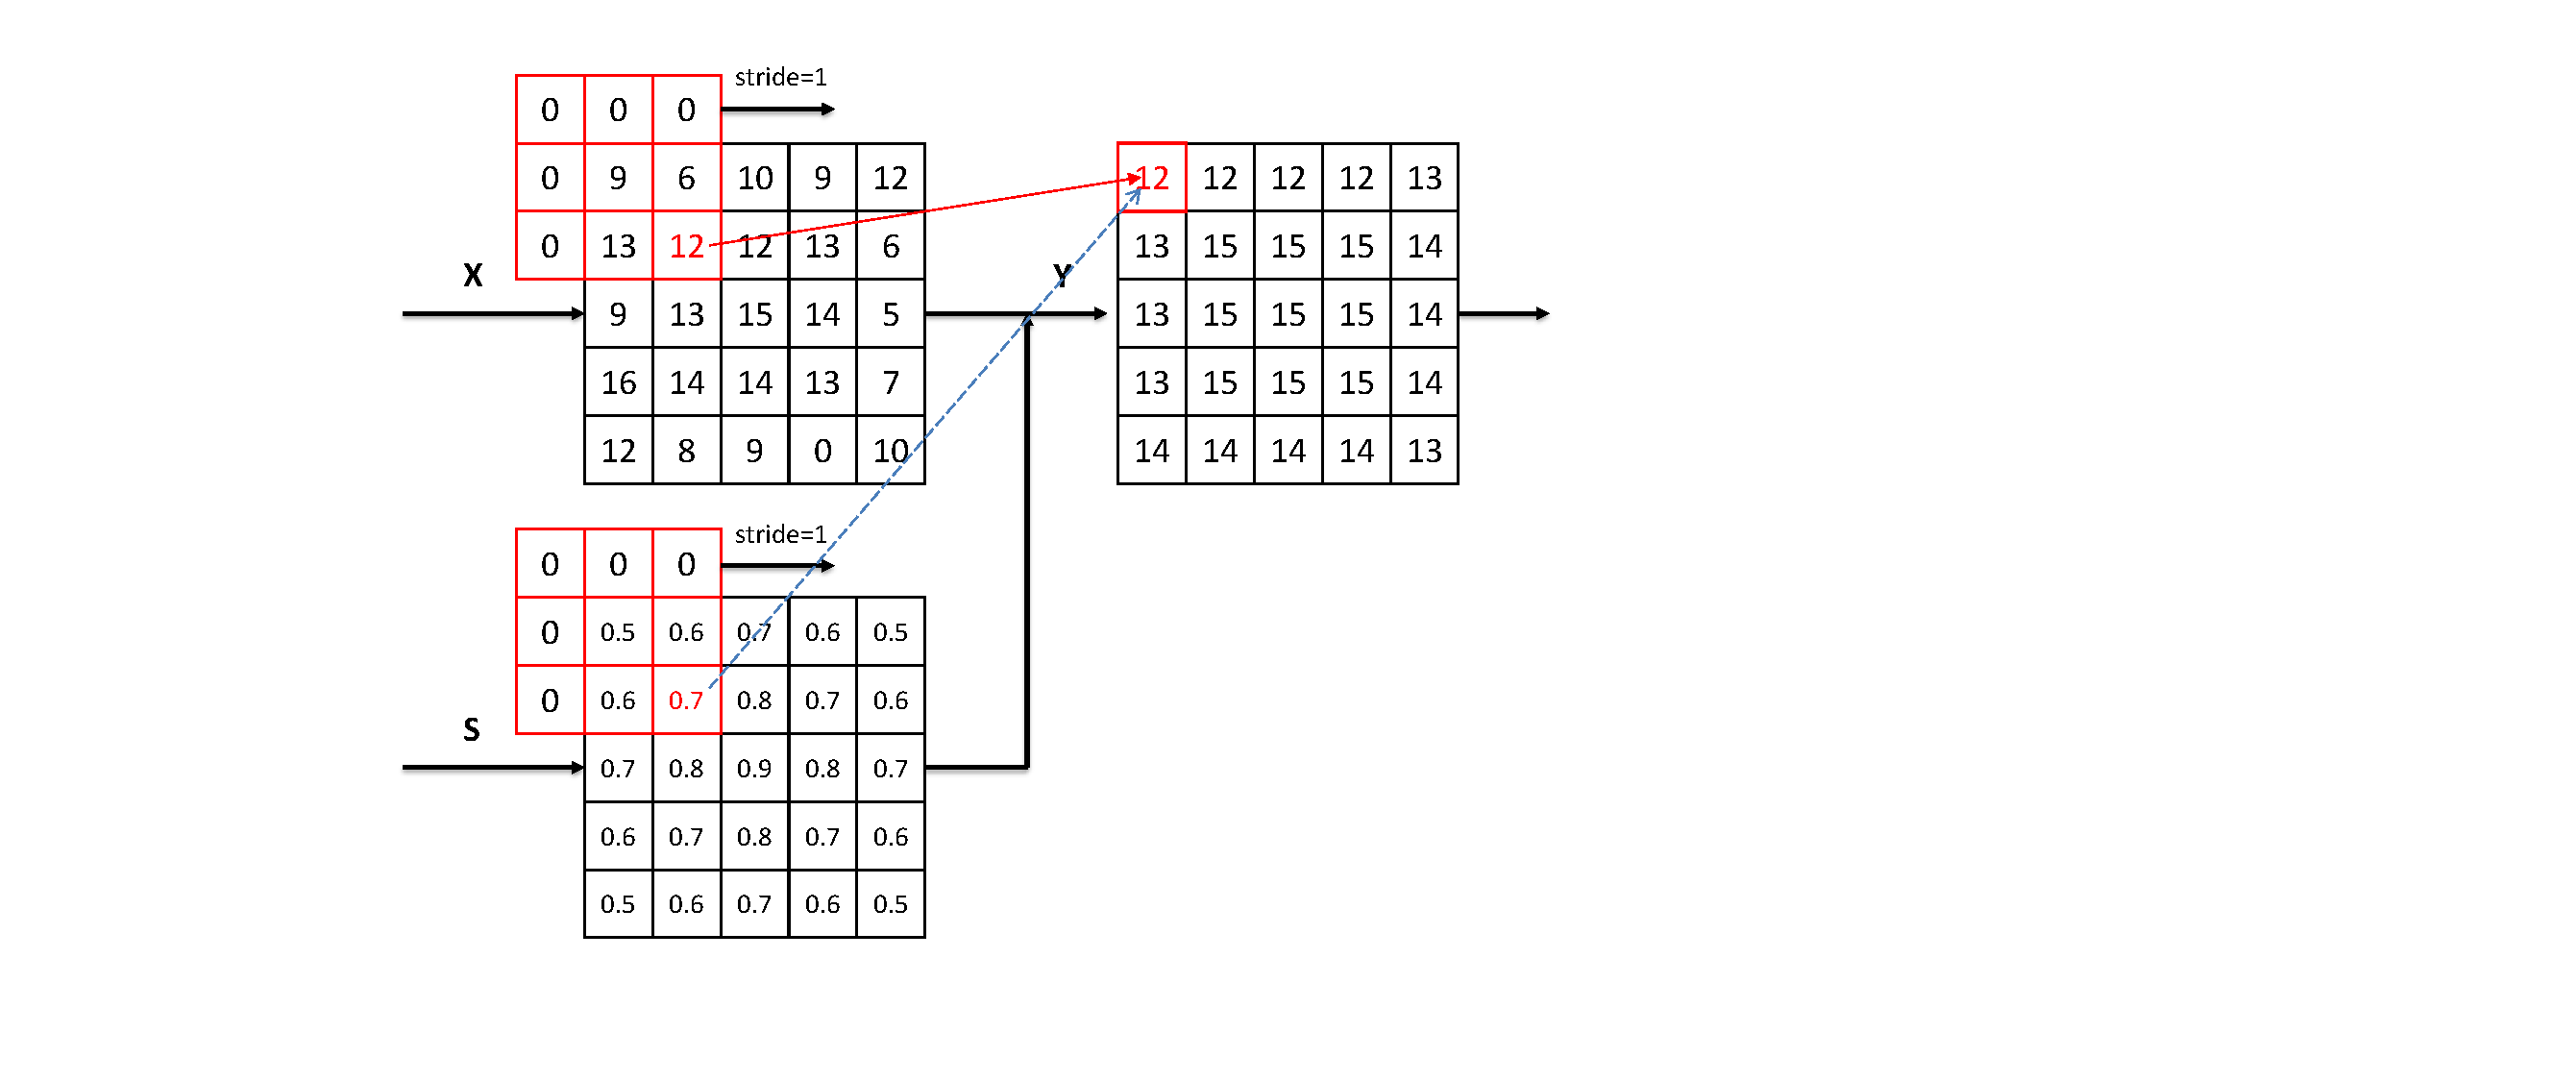
\includegraphics[width=3.4in]{Fig3.pdf}
   %\includegraphics[width=0.8\linewidth]{egfigure.eps}
\end{center}
   \caption{An example of joint max pooling.
   Two windows of same size synchronously slide on $\mathbf{X}$ and $\mathbf{S}$.
   Top window will propagate the element, of which the position corresponding to bottom window has a maximum value, to next layer.
   }
\label{F3}
\end{figure}
In practice, two windows with same size synchronously slide on two independent input.
One of the window is denoted as indicating window acting as the "indictor", while the other one is denoted as pooling windows, of which the useful information should be propagated to next layer.
In other word, elements in indicating window determine the pooling strategy in pooling windows.
A simple example is illustrated in Figure \ref{FigJMP}.

However for max pooling, $\mathbf{S}$ is hard to be directly learnt to be binary.
Therefore we add a threshold function by:
\begin{eqnarray}\label{jmp}
\begin{aligned}
y_{\mu,\nu} &= \sum_{i,j}x_{i,j}G(s_{i,j})~~~~x_{i,j}\in \mathbf{\overline{X}},s_{i,j}\in \mathbf{S} \\
G_{\mathbf{S}}(s_{i,j},)&=\left\{\begin{array}{cc}
1&if~s_{i,j}>=max(\mathbf{S})\\
0&else\\
\end{array}\right.
\end{aligned}
\end{eqnarray}

From Figure \ref{FigJMP}, it should be noted that most elements in $\mathbf{X}$ have been substituted with the element of which the position corresponding to maximum in $\mathbf{S}$.
Therefore in SCNN, if $\mathbf{O}_{seg}$ is denoted as $\mathbf{S}$ and $\mathbf{O}_{aux}$ is denoted as $\mathbf{X}$, only the contour description in $\mathbf{O}_{aux}$ with a local maximum objectness in $\mathbf{O}_{seg}$ can be retained by JMP.
Moreover, the discarded elements in $\mathbf{O}_{aux}$ will be replaced by a nearest retained contour description when pooling stride is set to be $1$
And positions with local maximum objectness usually correspond to the center region of objects.
Especially, the kernel size and iterations of JMP determine how far a retained contour expression can be spread.
JMP guarantees the accuracy and consistency of contour description in ambiguous region of an object.

One important contribution of our JMP is that the residual error can be correctly back propagated to its inputs.
This makes it a trainable layer in any network architecture and our SCNN become a fully trainable system.
Defining $L_\mathbf{X}$ as the residual error on $\mathbf{X}$ , the back propagation for $x_{i,j}$ can be expressed by:
\begin{eqnarray}\label{bpx}
\begin{aligned}
\frac{\partial L_\mathbf{X}}{\partial x_{i,j}}=\frac{1}{m}\sum\limits_{y_{\mu,\nu}\in\mathbf{U}}\frac{\partial L_\mathbf{X}}{\partial y_{\mu,\nu}}G_{\mathbf{S}_{u,v}}(s_{i,j})\\
\end{aligned}
\end{eqnarray}
where $\mathbf{U}$ is output set $\{y_{\mu.\nu}\}$ associated with $x_{i,j}$ and $m$ is the size of $\mathbf{U}$.
${S}_{u,v}$ is the corresponding pooling window centered on ${u,v}$ of $\mathbf{X}$.
Different from conventional max pooling, Eq. \ref{bpx} converge the gradients on the positions with local maximum $s_{i,j}$�� which usually are the centers of object.
Implementing Eq. \ref{bpx} to our SCNN can make it only focus on predicting accurate parameterized contour description on the center area of objects, instead of the whole region.


%Specially in Figure \ref{FigSCNN}, the input segmentation map is assumed to not only influence the output but also feeds a subsequent layers, thus also receiving gradient contributions $\frac{\partial L}{\partial s_{i,j}}$ from the next layer during back-propagation.

Defining $L_\mathbf{S}$ as the residual error on $\mathbf{S}$.
We assume that $s_{i,j}$ not only influences the following $y_{i,j}$ but also feeds a subsequent layer in Figure \ref{FigSCNN}, thus also receiving gradient contributions $\frac{\partial L_\mathbf{S}}{\partial s_{i,j}}$ from that layer during back-propagation.
The back propagation for $s_{i,j}$ is formulated by.
\begin{eqnarray}\label{bps}
\begin{aligned}
\frac{\partial L_\mathbf{S}}{\partial s_{i,j}}&=\frac{\partial L_\mathbf{S}}{\partial s_{i,j}}+\frac{1}{m}\sum_{y_{\mu,\nu}\in\mathbf{U}}\frac{\partial L_\mathbf{X}}{\partial y_{\mu,\nu}}\frac{\partial y_{\mu,\nu}}{\partial s_{i,j}}\\
&=\frac{\partial L_\mathbf{S}}{\partial s_{i,j}}+\frac{1}{m}\sum_{y_{\mu,\nu}\in\mathbf{U}}\frac{\partial L_\mathbf{X}}{\partial y_{\mu,\nu}}x_{i,j}\frac{\partial G_{\mathbf{S}_{u,v}}(s_{i,j})}{\partial s_{i,j}}\\
&=\frac{\partial L_\mathbf{S}}{\partial s_{i,j}}+\sum_{y_{\mu,\nu}\in\mathbf{U}}\frac{1}{m}\frac{\partial L_\mathbf{X}}{\partial y_{\mu,\nu}}x_{i,j}\delta_{\mathbf{S}_{u,v}}(s_{i,j})\\
\end{aligned}
\end{eqnarray}
where $\delta_{\mathbf{S}_{u,v}}(s_{i,j})$ is the derived function of $G_\mathbf{S}(s_{i,j})$, which has an infinite response when $s_{i,j}=max(\mathbf{S}_{u,v})$.
In order to normally back propagate, $\frac{\partial L_\mathbf{S}}{\partial s_{i,j}}$ is approximated by:
\begin{eqnarray}\label{dG}
\begin{aligned}
\frac{\partial L_\mathbf{S}}{\partial s_{i,j}}&= \frac{\partial L_\mathbf{S}}{\partial s_{i,j}}(1+\frac{1}{m}\sum_{y_{\mu,\nu}\in\mathbf{U}}\lambda\widetilde{\delta}_{\mathbf{S}_{u,v}}(s_{i,j}))\\
\widetilde{\delta}_{\mathbf{S}_{u,v}}(s_{i,j})&=\left\{\begin{array}{cc}
1&if~s_{i,j}=max(\mathbf{S})\\
0&else\\
\end{array}\right.
\end{aligned}
\end{eqnarray}

Intuitively, Eq. \ref{dG} add a loss weight on gradients of local maximum $s_{i,j}$ with the control $\lambda$ (set according to iterations of JMP) to avoid false detection as much as possible.
\subsection{Fusion for Final Segmentation}
With the predicted probability maps of objectness $\mathbf{O}_{seg}$ and parameterized contour description $\mathbf{O}_{aux}$ from SCNN, the final segmentation $m(i,j)$ can be obtained by fusing them together:
\begin{eqnarray}\label{fusion}
\begin{aligned}
m(i,j)=\left\{\begin{array}{cc}
1&if~\mathbf{O}_{seg}(i,j)>\tau_2\\
0&if~\mathbf{O}_{seg}(i,j)<\tau_1\\
f(\mathbf{O}_{aux}(i,j))&else\\
\end{array}\right.
\end{aligned}
\end{eqnarray}
where $\tau_2$ and $\tau_1$ are the thresholds (set empirically) to control the degree of object contour modification by $\mathbf{O}_{aux}(i,j)$.
$f(\mathbf{O}_{aux}(i,j))$ is a function judging whether a position is within a shape by its coordinate $(i,j)$ and shape description $\mathbf{O}_{aux}(i,j)$.
For example in our task, we define an ellipse by $\mathbf{O}_{aux}(i,j) = [\theta, x_c, y_c, a, b]$, therefore the function is expressed by:
\begin{eqnarray}\label{fusion}
\begin{aligned}
f(\mathbf{O}_{aux}(i,j))&=\left\{\begin{array}{cc}
1&if~\frac{dx^2}{a^2}+\frac{dy^2}{b^2}<1\\
0&else\\
\end{array}\right.\\
dx &= cos(\theta)(i-x_c)+sin(\theta)(j-y_c)\\
dy &= -sin(\theta)(i-x_c)+cos(\theta)(j-y_c)\\
\end{aligned}
\end{eqnarray}

Our fusion strategy can appropriately utilize prior shape knowledge to optimize segmented object.
It can not only separate objects into individual ones, but also optimize most regular object while don't loss generalization to deformable objects.
The SCNN can be easily extended to other shape constraint, if only the shape can be parameterized.

\section{Experiments}
We first present results on two diverse biomedical image segmentation problems to demonstrate our superiority over existing methods.
The applications including synaptic vesicle segmentation and gland segmentation.
Additionally, our SCNN is extended to scene text segmentation task to prove its generic applicability.

\subsection{Synaptic vesicle segmentation}
\textbf{Dataset}
Synaptic vesicle is a good example to evaluate our method.
The images were acquired by .
They are much noisy and contain both vesicle and ambiguous membrane structure, such as cell nucleus.
%The ground truths of dataset are held out by biologists for objective evaluation.
The dataset is composed of $8787$ images with ground truth annotations provided by biologists.
[copy]To increase the robustness and reduce overfitting,
we utilized the strategy of data augmentation to enlarge the training dataset.
The augmentation transformations include translation, rotation and flipping.[copy]
For cross validation experiments, The dataset are divided into two parts.
The first five out of six images are prepared to train our model and the rest of them are used to test its performance.
The validation processing has been repeated several times and the average performance will be reports.

\textbf{Implementation details}
[copy]Our framework was evaluated on the open-source deep learning library Caffe \cite{Jia2014}[copy].
The network resize the image to $321\times 321$ as input and output objectness score and parameterized contour maps.
[copy]A three-step training process is employed.
We first train the segmentation branch independently and then we jointly fine-tune the multi-task network without joint max pooling.
[copy]Specifically, we employ exactly the same setting as \cite{Chen2014a} in the first stage.[copy]
In the second stage, the balancing weight $\lambda$ is set to be $5$ and a small learning rate of $10^{-8}$ is employed for fine-tuning in the second stage.
In the final stage, the joint max pooling is attached to the tail of network and the whole model is fine-tuned again to further improve the performance.
In order to make better use of parameterized contour information, the joint max pooling is iterated twice with the pooling size $11\times 11$ and stride $1$.
Finally in fusion step as most vesicle contours shape are regular, $\tau_2$ and $\tau_1$ are set to be $0.9$ and $0.2$ for a strong modification by parameterized contour constraint.

\textbf{Evaluation setup}
The evaluation criteria in our experiments includes F1 score and pixel intersection-overunion (IOU) averaged across different classes.
The F1 score considers the performance of object detection, while IOU consider the segmentation performance, respectively.

For detection, the metric F1 score is defined as:
\begin{eqnarray}\label{fusion}
\begin{aligned}
F1 = \frac{2PR}{P+R},P=\frac{N_{tp}}{N_{tp}+N_{fp}},R=\frac{N_{tp}}{N_{tp}+N_{fn}}
\end{aligned}
\end{eqnarray}
where $M_{tp}$,$M_{fp}$ and $M_{fn}$ are respectively the number of true positives, false positives and false negatives.
Especially, a segmented object that intersects with at least 50 with the ground truth is regarded as a true positive, otherwise it is regarded as a false positive.
If a ground truth object has no corresponding segmented object that intersects more than 50, it is regarded as a false negative.

For segmentation, the metric IOU is defined as:
\begin{eqnarray}\label{fusion}
\begin{aligned}
IOU = \frac{1}{N_s}\sum_{i=1}^{N_s}\frac{G_i\bigcap S_i}{G_i\bigcup S_i}
\end{aligned}
\end{eqnarray}
where $N_i$ denotes the number of segmented classes.
$G_i$ denotes the ground truth of $i$-th class.
$S_i$ denotes the segmented map of $i$-th class.

\textbf{Qualitative evaluation on vesicle segmentation}
Figure \ref{} shows some segmentation results of testing data.
In order to verify the effectiveness of parameterized contour information, we compared the performance of u-net \cite{Ronneberger2015} relying only on the prediction of vesicle objects and DCAN \cite{Chen2016a} using contour probability information.
From segmentation results we can see that without any complementary information, there exists many touching vesicle objects that cannot be separated by u-net.
This situation usually occurs in regions with ambiguous context between two vesicle objects.
And the contours of many regular objects are very coarse, as the case shown in the second row of Figure \ref{}.
Although DCAN is capable of separating the touching vesicles into individuals in the third row in Figre \ref{}, the obtained contours of regular vesicle are still coarse.
In comparison, our SCNN using the parameterized contour information can not only separate those touching vesicles clearly, but also obtain a much smooth and regular shape for each vesicle contour.
This demonstrates the superiority of our SCNN in segmenting densely arranged objects with regular shape contour by exploring the complementary information in parameterized contour descripition.


\textbf{Quantitative evaluation}
We used metrics of F1 score and IOU to evaluate our method.
We compare SCNN with the state of the art segmentation methods based on Deeplab \cite{Chen2014a}, U-net \cite{Ronneberger2015} and DCAN \cite{Chen2016b}, which are commonly used in biomedical image process.
Their results on our synaptic vesicle dataset are shown in \ref{tab:vesicle}.
And we further implement two version of SCNN.
The first SCNNv1 is the implementation of multi-task neural network without joint max pooling, and SCNNv2 is the complete form.
Their results are also presented in Table \ref{tab:vesicle} to prove effectiveness of our joint max pooling.

Qualitatively, the performance of SCNN surpassed all the other methods by a large margin on vesicle segmentation task, proving its effectiveness for segmenting regular biomedical objects.
From Table \ref{}, we can find that

\begin{table}\label{tab:vesicle}
\begin{center}
\begin{tabular}{lcc}
\hline
Method & F1 & IOU \\
\hline
DeepLab & 0.8404 & 0.8495 \\
U-net & 0.8404 & 0.8495 \\
DCAN & 0.8404 & 0.8495 \\
SCNNv1 & 0.8404 & 0.8495 \\
SCNNv2 & 0.8404 & 0.8495 \\
\hline
\end{tabular}
\end{center}
\caption{The detection and segmentation results of different methods in our synaptic vesicle segmentation dataset.}
\end{table}
\subsection{Gland segmentation}
\textbf{Dataset}
In this section we present SCNN for segmenting benign and malignant gland.
We consider the public dataset of $Gland$ $Segmentation$ $Challenge$ $Contest$ in MICCAI2015 \cite{Sirinukunwattana2015a}
The training dataset is composed of 85 images, consisting of 37 benign and 48 malignant, with ground truth annotations provided by expert pathologists.
Especially, there is a huge variation of glandular morphology in malignant case, which can prove the generalization of our SCNN to irregular objects.
The same data augmentation in vesicle segmentation is implemented for a better performance.

\textbf{Implementation details}
Because there exists many irregular objects in gland images that we desire to remain more contour information obtained by object prediction, the contour modification by parameterized contour information should be relatively weaker than segmenting vesicles.
By experimental verification, we find that $\tau_2=$ 0.7 and $\tau_1 = $0.4 produce a better results.
And we still use the standard elliptic parameter as the prior shape constraint for gland, as most benign glands and few malignant glands' shape are approximate ellipses.
The other implementation settings and evaluation metrics follow the vesicle segmentation.

\textbf{Qualitative evaluation on gland segmentation}
Follow previous qualitative evaluation, we presented the results of u-net and the state of art method DCAN in gland segmentation with our SCNN in Figure \ref{}.
The first two column are the examples of benign gland images, and the rest two column are the examples of malignant images.
From the results, we can observed that both SCAN and SCNN can well solve the touching problem in benign and malignant cases.
However for benign case, the contours of glands obtained by SCNN are more smooth than that of DCAN.
And for malignant case, since SCNN only modify the segmentation predictions on the object border, there is no obvious deterioration compared to DCAN.



\textbf{Quantitative evaluation}
Table \ref{} shows the F1 score and IOU metric over the $Gland$ $Segmentation$ $Challenge$ $Contest$ by several commonly used biomedical segmentation methods.

\subsection{Scene text detection}
We further extended SCNN to scene text detection task, which


{\small
\bibliographystyle{ieee}
\bibliography{egbib}
}

\end{document}
